\chapter{Construcciones}%
\label{cha:construcciones}
En este capítulo buscaremos topologías en base a unas aplicaciones con el objetivo de hacer a dichas aplicaciones continuas. Tras esto, daremos una caracterización de la topología construida. Por último, exploraremos las propiedades de las construcciones.

\section{Imágenes inversas}%
\label{sec:imagenes_inversas}
Supongamos que tenemos $f: Y \rightarrow \left( X, \mathcal{T} \right)$ y buscamos hacerla continua. Trivialmente, podemos hacer que la topología en $Y$ sea la discreta, sin embargo, esto carece de interés. Por esta razón, buscamos la topología \underline{menos fina} que haga $f$ continua. 
\begin{defi}    
Llamamos \textbf{topología de la imagen inversa} a: $f^{-1} \mathcal{T} = \{f^{-1}U: U \in \mathcal{T}\}$.
\end{defi}
\begin{prop}    
La topología de la imagen inversa cumple:
\begin{enumerate}
    \item Es topología. 
    \item Es mínima. 
\end{enumerate}
\end{prop}
%TODO: Acabar
\begin{demo}
\begin{enumerate}
    \item Trivial.
    \item Sea $\mathcal{T}'$ otra topología en $Y$ que haga $f$ continua. 

    Tomamos $U \in f^{-1}\mathcal{T} \Rightarrow \exists V \in \mathcal{T}: f^{-1}V = U$. Como $f$ en $\mathcal{T}'$ es también continua tenemos que $U = f^{-1}V$ es abierto en $\mathcal{T}'$. Es decir, todo abierto en $f\mathcal{T}$ es también abierto en $\mathcal{T}' \Rightarrow \boxed{f \mathcal{T} \subset \mathcal{T}'}$.
\end{enumerate}
\end{demo}

\begin{obs}
    Con esta definición, $f$ será continua.
\end{obs}

\subsection{Caracterización de la imagen inversa}
\label{sub:caracterizacion_de_la_imagen_inversa}
Veamos ahora una caracterización de la topología que acabamos de introducir.
\begin{theo}[Propiedad universal de las inmersiones]
Sean $g: \left( Z, \mathcal{T}'' \right) \rightarrow \left( Y, \mathcal{T}' \right)$ y $f: \left( Y, \mathcal{T}' \right) \rightarrow \left( Z, \mathcal{T} \right)$. Entonces:
    \[
    \mathcal{T}' = f^{-1}\mathcal{T} \Leftrightarrow  
    \]
    \begin{equation}\label{ec:prop_universal_inm}
        \left[\forall g: g \text{ cont.} \Leftrightarrow f \circ g \text{ cont.} \right]  
    \end{equation}

    \begin{figure}[H]
        \centering    
            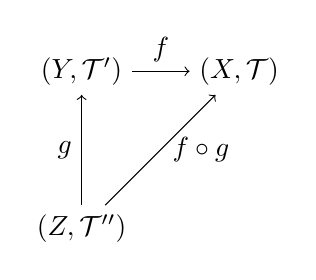
\begin{tikzpicture}[node distance=2cm, auto]
            \node(Y) {$\left( Y, \mathcal{T}' \right)$};
            \node(X) [right of=Y] {$\left( X, \mathcal{T} \right)$};
            \node(Z) [below of=Y] {$\left( Z, \mathcal{T}'' \right)$};
            \draw[->](Y) to node {$f$}(X);
            \draw[->](Z) to node [left] {$g$}(Y);
            \draw[->](Z) to node [right=0.2ex] {$f \circ g$}(X);
            \end{tikzpicture}
        \caption{\textit{Ilustración de la composición propuesta}}
        \label{prop_universal_inmersiones}
    \end{figure}
\end{theo}
\begin{demo}
\begin{itemize}
    \item $\Rightarrow)$ $\mathcal{T}' = f^{-1}\mathcal{T}: $ 
    \begin{itemize}
        \item $g$ cont. $\Rightarrow f \circ g$ cont. (Composición de continuas)
        \item $f \circ g$ cont. $\Rightarrow g$ cont. ($V \in \mathcal{T}' \Rightarrow g^{-1}V \stackrel{\mathcal{T}' = f^{-1}\mathcal{T}}{=} g^{-1} f^{-1}U = \left( f \circ g \right)^{-1} U \stackrel{f \circ g \text{ cont.}}{\in} \mathcal{T}''$)
    \end{itemize}

    \item $\Leftarrow)$ Por otro lado, veamos la unicidad:
    \begin{figure}[H]
        \centering    
            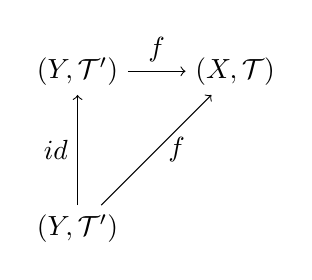
\begin{tikzpicture}[node distance=2cm, auto]
            \node(Y) {$\left( Y, \mathcal{T}' \right)$};
            \node(X) [right of=Y] {$\left( X, \mathcal{T} \right)$};
            \node(Z) [below of=Y] {$\left( Y, \mathcal{T}' \right)$};
            \draw[->](Y) to node {$f$}(X);
            \draw[->](Z) to node [left] {$id$}(Y);
            \draw[->](Z) to node [right=0.2ex] {$f$}(X);
            \end{tikzpicture}
    \end{figure}
    Como esta $id$ es continua, por (\ref{prop_universal_inmersiones}), $f\circ id = f$ es también continua. Al ser $f^{-1}\mathcal{T}$ la menos fina, $\mathcal{T}' \supset f^{-1}\mathcal{T}$.

    Además, 
    \begin{figure}[H]
        \centering    
            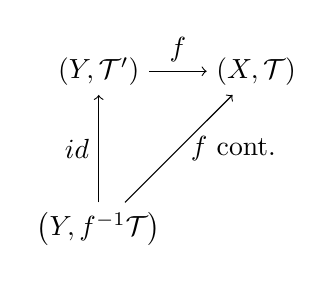
\begin{tikzpicture}[node distance=2cm, auto]
            \node(Y) {$\left( Y, \mathcal{T}' \right)$};
            \node(X) [right of=Y] {$\left( X, \mathcal{T} \right)$};
            \node(Z) [below of=Y] {$\left( Y, f^{-1}\mathcal{T} \right)$};
            \draw[->](Y) to node {$f$}(X);
            \draw[->](Z) to node [left] {$id$}(Y);
            \draw[->](Z) to node [right=0.2ex] {$f$ cont.}(X);
            \end{tikzpicture}
    \end{figure}
    Como la $f$ es continua, por (\ref{prop_universal_inmersiones}), esta nueva $id$ es también continua $\Rightarrow f^{-1}\mathcal{T} \supset \mathcal{T}'$.
\end{itemize}
\end{demo}

\begin{enun}
Demostrar $\Leftarrow$) sin usar que $f^{-1}\mathcal{T}$ es la menos fina (usar que cumple la caracterización). Hecho en clase.
\end{enun}

\subsection{Inmersiones}
\label{sub:inmersiones}
Veamos ahora un caso de especial relevancia:
\[
\boxed{f: Y \rightarrow X \text{ inyectiva}} 
\]
\begin{defi}
Una aplicación continua \underline{inyectiva} $f: \left( Y, \mathcal{T}' \right) \rightarrow \left( X, \mathcal{T} \right)$ tal que $\mathcal{T}' = f^{-1} \mathcal{T}$ se llama \textbf{inmersión}.
\end{defi}

\begin{prop}
Sea $f: \left( Y, \mathcal{T}' \right) \rightarrow \left( f\left( Y \right), \mathcal{T} \right)$. Entonces:
\[
    \mathcal{T}' = f^{-1}\mathcal{T} \Leftrightarrow f: \left( Y, \mathcal{T}' \right) \xrightarrow{\text{homeo.}} \left( f\left( Y \right), \mathcal{T}|_{f\left( Y \right)} \right)
\]
\end{prop}
\begin{demo}
\begin{itemize}
    \item $\Rightarrow)$ Tenemos que $f: \left( Y, f^{-1}\mathcal{T} \right) \rightarrow \left( f\left( Y \right), \mathcal{T}|_{f\left( Y \right)} \right)$. 

    Al ser $f$ inyectiva, también será biyectiva. Veamos que es continua y abierta:
    \begin{itemize}
        \item \underline{Continua}: Sea $U \in \mathcal{T}|_{f\left( Y \right)} \Rightarrow \exists W \in \mathcal{T}: U = f\left( Y \right) \cap W \Rightarrow$ 
        \[
        f^{-1}\left( U \right) = f^{-1}\left( W \cap f\left( Y \right) \right) = Y \cap f^{-1}\left( W \right) = f^{-1}\left( W \right)
        \]
        que es abierto en $f^{-1}\mathcal{T}$.
        \item \underline{Abierta}: Sea $U \in f^{-1}\mathcal{T} \Rightarrow \exists W \in \mathcal{T}: f^{-1}W = U$. Aplicando $f$:
        \[
        fU = ff^{-1}W = W \cap f\left( Y \right) \stackrel{\text{ab.}}{\subset} f\left( Y \right)
        \]
        es decir que $fU$ es abierto en $f\left( Y \right)$.
    \end{itemize}

    %TODO: Posiblemente mal. Algo de la relativa 
    \item $\Leftarrow)$ Veamos la doble contención:
    \begin{itemize}
        \item $\subset)$ Sea $U \in \mathcal{T}' \xRightarrow{\text{ab.}} fU \in \mathcal{T}|_{f\left( Y \right)}$, es decir, $\exists W \in \mathcal{T}'|_{f\left( Y \right)}: f^{-1}W = U$. Por tanto, $U \in f^{-1}\mathcal{T}$. 
        \item $\supset)$ Sea $U \in f^{-1}\mathcal{T} \xRightarrow{\text{def.}} \exists W \in \mathcal{T}|_{f\left( Y \right)}: f^{-1}W = U$. Como $f$ es continua en $\mathcal{T}'$, $U = f^{-1} W \in \mathcal{T}'$.
    \end{itemize}
\end{itemize} 
\end{demo}

%TODO: No se si es necesario
\begin{obs}
\begin{enumerate}
    %TODO: Igual al anterior?
    \item $f: Y \rightarrow X$ $1-1$ cont. $+ \begin{cases}
        \text{abierto} \Rightarrow \text{inmersión }\\
        \text{cerrado} \Rightarrow \text{inmersión } 
    \end{cases}$
    \begin{demo}
        \begin{itemize}
            \item Abierto en $X \Rightarrow$ abierto en $f\left( Y \right)$.
            \item Cerrado en $X \Rightarrow$ cerrado en $f\left( Y \right)$.
        \end{itemize}
    \end{demo}

    \item $f: Y \rightarrow X$ inmersión: $\begin{cases}
        \text{abierto } \Leftrightarrow f\left( Y \right) \text{abierto en } X\\
        \text{cerrado } \Leftrightarrow f\left( Y \right) \text{cerrado en } X\\
    \end{cases}$
    \begin{demo}
    \begin{itemize}
        \item 
        $f\left( Y \right) \stackrel{\text{ab.}}{\subset} X: V = f^{-1}U \in f^{-1}\mathcal{T} \Rightarrow fV = \overbrace{U \cap f\left( Y \right)}^{\text{inter. abiertos}} \in \mathcal{T}$.
        \item 
        $f\left( Y \right) \stackrel{\text{cerr.}}{\subset} X: C \stackrel{\text{cerr.}}{\subset}  f^{-1}\mathcal{T} \Rightarrow Y\setminus C = f^{-1} U \in f^{-1}\mathcal{T} \Rightarrow f\left( C \right) = \underbrace{\left( X\setminus U \right) \cap f\left( Y \right)}_{\text{inter. cerrados}}  \stackrel{\text{cerr.}}{\subset} X$ 
    \end{itemize} 
    \end{demo}

    \item Tenemos como posibilidades: 
    \begin{itemize}
        \item Inmersión $ + \not$ ab. $+ \not$ cerr.
        \item Inmersión $+$ ab. $+ \not $ cerr.
        \item Inmersión $+ \not$ ab. $+$ cerr.
    \end{itemize}
\end{enumerate}
\end{obs}

\begin{obs}
Las inmersiones permiten considerar unos espacios como subespacios de otros. Las frases ``el plano proyectivo real no es un subespacio de $\mathbb{R}^3$'', ``la esfera no es un subespacio de $\mathbb{R}^2$'', ``el plano proyectivo real es un subespacio de $\mathbb{R}^4$'' se refieren a esto: \underline{cuándo hay o no hay} una inmersión del primer espacio en el segundo, es decir, un subespacio del segundo homeomorfismo al primero. Es un problema fundamental de la topología
y de la geometría.
\end{obs}


\section{Imágenes directas}%
\label{sec:imagenes_directas}
Supongamos que tenemos $f: \left( X, \mathcal{T} \right) \rightarrow Y$ y buscamos hacerla continua. Trivialmente, podemos hacer que la topología en $X$ sea la trivial, sin embargo, esto carece de interés. Por esta razón, buscamos la topología \underline{más fina} que haga $f$ continua.

\begin{defi}
Llamamos \textbf{topología de la imagen directa} a: $f\mathcal{T} = \{V \subset Y: f^{-1}V \in \mathcal{T}\}$.
\end{defi}
\begin{prop}    
\begin{enumerate}
    \item Es topología.
    \item Máxima. 
\end{enumerate}
\end{prop}
\begin{demo}
\begin{enumerate}
    \item Trivial.
    \item Sea $\mathcal{T}'$ tal que haga $f$ continua. Veamos que $\mathcal{T}' \subset f\mathcal{T}$.

    Tomamos $U \in \mathcal{T}' \Rightarrow \exists W \in \mathcal{T}': f^{-1} U = W$. Por definición de $f \mathcal{T}$, ya tenemos que $U \in f \mathcal{T}$ (porque $W \in Y$).
\end{enumerate}
\end{demo}
\begin{obs}
Con esta definición, $f$ será continua.
\end{obs}

\subsection{Caracterización de la imagen directa}
\label{sub:caracterizacion_de_la_imagen_directa}
Veamos ahora una caracterización de la topología que acabamos de introducir.
\begin{theo}[Propiedad universal de las identificaciones]
Sean $g: \left( Y, \mathcal{T}' \right) \rightarrow \left( Z, \mathcal{T}'' \right)$ y $f: \left( X, \mathcal{T} \right) \rightarrow \left( Y, \mathcal{T}' \right)$. Entonces:
    \[
    \mathcal{T}' = f\mathcal{T} \Leftrightarrow  
    \]
    \begin{equation}\label{eq:prop_universal_directa}
        \forall g \left[ g \text{ cont.} \Leftrightarrow g \circ f \text{ cont.} \right]
    \end{equation}

    \begin{figure}[H]
        \centering    
            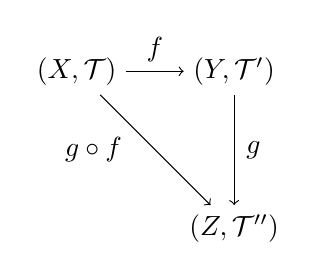
\begin{tikzpicture}[node distance=2cm, auto]
            \node(X) {$\left( X, \mathcal{T} \right)$};
            \node(Y) [right of=X] {$\left( Y, \mathcal{T}' \right)$};
            \node(Z) [below of=Y] {$\left( Z, \mathcal{T}'' \right)$};
            \draw[->](X) to node {$f$}(Y);
            \draw[->](X) to node [left=0.3cm] {$g \circ f$}(Z);
            \draw[->](Y) to node [right=0.2ex] {$g$}(Z);
            \end{tikzpicture}
        \caption{\textit{Ilustración de la composición propuesta}}
        \label{prop_universal_directas}
    \end{figure}
\end{theo}
\begin{demo}
\begin{enumerate}
    \item $\mathcal{T}' = f^{-1}\mathcal{T}: $ 
    \begin{itemize}
        \item $g$ cont. $\Rightarrow g \circ f$ cont. (Composición de continuas)
        \item $g \circ f$ cont. $\Rightarrow g$ cont. ($W \in \mathcal{T}'' \Rightarrow f^{-1}\left( g^{-1} W \right) = \underbrace{\left( g \circ f \right)^{-1}}_{\text{cont.}} W \in \mathcal{T} \stackrel{\mathcal{T}' = f\mathcal{T}}{\Rightarrow} g^{-1}W \in \mathcal{T}'$)
    \end{itemize}

    \item Por otro lado, veamos la unicidad:

    \begin{figure}[H]
        \centering    
            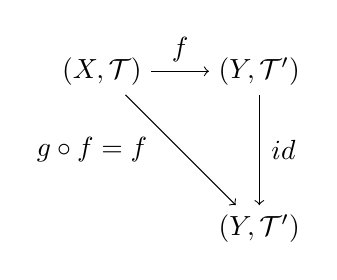
\begin{tikzpicture}[node distance=2cm, auto]
            \node(X) {$\left( X, \mathcal{T} \right)$};
            \node(Y) [right of=X] {$\left( Y, \mathcal{T}' \right)$};
            \node(Z) [below of=Y] {$\left( Y, \mathcal{T}' \right)$};
            \draw[->](X) to node {$f$}(Y);
            \draw[->](X) to node [left=0.3cm] {$g \circ f = f$}(Z);
            \draw[->](Y) to node [right=0.2ex] {$id$}(Z);
            \end{tikzpicture}
    \end{figure}
    Como $id$ será continua, aplicamos \ref{eq:prop_universal_directa} y tenemos que $g \circ f = f$es continua. Al ser $f \mathcal{T}$ la más fina $\Rightarrow \mathcal{T}' \subset f \mathcal{T}$.

    \begin{figure}[H]
        \centering    
            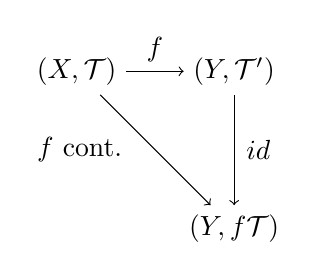
\begin{tikzpicture}[node distance=2cm, auto]
            \node(X) {$\left( X, \mathcal{T} \right)$};
            \node(Y) [right of=X] {$\left( Y, \mathcal{T}' \right)$};
            \node(Z) [below of=Y] {$\left( Y, f\mathcal{T} \right)$};
            \draw[->](X) to node {$f$}(Y);
            \draw[->](X) to node [left=0.3cm] {$f$ cont.}(Z);
            \draw[->](Y) to node [right=0.2ex] {$id$}(Z);
            \end{tikzpicture}
    \end{figure}
    Como $f$ es continua por definición de $f \mathcal{T}$, aplicamos \ref{eq:prop_universal_directa} y tenemos que esta $id$ es continua. Por esta razón, $f \mathcal{T} \subset \mathcal{T}'$.
\end{enumerate}
\end{demo}

\begin{enun}    
Demostrar (ii) sin usar que $f\mathcal{T}$ es la más fina (usar que cumple la caracterización)
\end{enun}

\begin{obs}
$f\left( X \right)$ es abierto y cerrado en $f\mathcal{T}: \begin{cases}
    \forall y \in Y \setminus f\left( X \right), f^{-1}y = \emptyset \in \mathcal{T} \Rightarrow \{y\} \in f\mathcal{T}\\
    f^{-1}f\left( X \right) = X \in \mathcal{T} \Rightarrow f\left( X \right) \in f\mathcal{T}
\end{cases}$
\end{obs}

%TODO: En sus apuntes el orden es distinto a como lo dio en clase. De momento, lo dejo como en los apuntes.
\subsection{Identificaciones}
\label{sub:identificaciones}
Veamos ahora un caso de especial relevancia:
\[
\boxed{f: X \rightarrow Y \text{ sobreyectiva}.} 
\]
%TODO: No sé de donde viene esto. Explicar el interés de este caso. f(X) nos dirá todo lo necesario.
Para entender los abiertos de una imagen directa es conveniente representarlos en el dominio. El concepto es conjuntista en realidad:

\subsubsection*{Conjuntos saturados}
Conjuntos saturados\begin{defi}
Un conjunto $A \subset X$ es \textbf{saturado} (respecto de $f$) si $f^{-1}f\left( A \right) = A$.
\end{defi}
\begin{prop}
Los abiertos de $f\mathcal{T}$ son las imágenes de los abiertos saturados de $\mathcal{T}$:
\[
U \in f \mathcal{T} \Leftrightarrow \exists W \in \mathcal{T}\text{, saturado}: fW = U.
\]
\end{prop}
\begin{demo}
\begin{itemize}
    %TODO: No sé si está del todo bien.
    \item $\Rightarrow)\ V \in f\mathcal{T} \Rightarrow f^{-1}V \in \mathcal{T}$ y $V \stackrel{f \text{ sobre}}{=} f^{-1}fV$, es decir, que $f^{-1} V$ es saturado.
    \item $\Leftarrow)$ Sea $V \in Y: \exists U \in \mathcal{T}$, saturado tal que: $fU = V$. Debemos ver que $f^{-1}V \in \mathcal{T}$.

    Como $f^{-1}V = f^{-1}fU \stackrel{\text{sat.}}{=} U \in \mathcal{T}$ ya lo tenemos.
\end{itemize}
\end{demo}

\begin{obs}
Los abiertos \underline{no} saturados de $X$ pueden tener imágenes \underline{no} abiertas de $Y$. 
\end{obs}

\begin{ej}
\begin{enumerate}
    %TODO: Hacer la circunferencia con todo R
    \item Sea:
    \begin{align*}
        f: \left[ 0, 1 \right] &\rightarrow \mathbb{S}^1 = Y\\ 
        t &\mapsto \underbrace{\left( \cos 2\pi t, \sin 2\pi t \right)}_{\exp\left( 2 \pi it \right)}
    \end{align*}
    que geométricamente es:
    \begin{figure}[H]
        \centering
        \begin{tikzpicture}
            %Flechas y texto
            \draw[gray] (0,0) -- (3,0); 
            \draw[green, ->] (0,0) -- (1,0); 
            \draw[green, ->] (3,0) -- (2,0); 
            \draw[red, ->] (3,0.4) -- (2.2,0.4); 
            \node[green] at (3.1,0.03) [right] {Saturado};
            \node[red] at (3.05,0.45) [right] {No saturado};

            %0 y 1
            \node[gray] at (0,0) [below] {$0$};
            \node[gray] at (0,0) {\textbullet};

            \node[gray] at (3,0) [below] {$1$};
            \node[gray] at (3,0) {\textbullet};

            %t saturado
            \node[gray] at (1.5,0.3) {$t$};
            \node[gray] at (1.5,0) {\textbullet};
            \node[gray] at (1.5,-0.3) {Saturado};

            %Paréntesis t
            \node[gray] at (1.3,0) {(};
            \node[gray] at (1.7,0) {)};

            \draw [gray, decorate, decoration = {brace}] (5.1,0.6) -- (5.1,-0.2);
            \node[gray] at (5.2,0.2) [right] {Abierto};

            %Función
            \node(X) at (-1,0) {$X$};
            \node(S) at (-1,-1.5) {$\mathbb{S}^1$};
            \draw[->](X) -- node [left] {$f$} (S);

            %Circulo 
            \draw[color=gray, very thick,
                decoration={markings, mark=at position 0.07 with \arrow[green]{)};,
                                      mark=at position 0.35 with \arrow{(};,
                                      mark=at position 0.47 with \arrow{)};,
                                      mark=at position 0.95 with \arrow[green]{(};,
                                      mark=at position 0.97 with \arrow[red]{(};,
                           },
                postaction={decorate}
                ] (1.5,-2) circle (1);
                %Centro
                \node(O) [gray] at (1.5,-2) {\textbullet};
                %Izquierda
                \node(izq) [gray] at (0.7,-1.4) {\textbullet};
                %Derecha
                \node(der) [gray] at (2.5,-2) {\textbullet};
                %Radio derecho
                \draw[gray, dashed] (O) -- (der);
                %Radio izquierdo
                \draw[gray, dashed] (O) -- (izq);
                
            %Entorno derecho
            \node[gray] at (der) [right] {$f\left( 0 \right) = f\left( 2 \pi \right)$};
            \node[green] at (2.5,-1.4) [right] {Es entorno abierto de $f\left( 0 \right)$};
            \node[red] at (2.5,-2.7) [right] {No es entorno abierto de $f\left( 0 \right)$};

            %Entorno izquierdo
            \node[gray] at (izq) [left] {$f\left( t \right)$};
            \draw[->, thick, gray] (-0.7,-2.3) -- (0.2,-1.8);
            \node[gray] at (0.5,-2.7) [left] {Entorno en $f \mathcal{T}$};

            %Localización
            \draw [gray, decorate, decoration = {brace}] (7.4,-1.1) -- (7.4,-3);
            \node[gray] at (7.5,-2.05) [right] {En $f\mathcal{T}$};
        \end{tikzpicture}
        \caption{\textit{La topología imagen directa es la usual en $\mathbb{S}^1$}}
        \label{fig:proyeccion_exponencial_img_directa}
    \end{figure}

    \item Tenemos:
    \begin{align*}
        f: R = \left[ 0, 1 \right] \times \left[ 0, 1 \right] &\rightarrow C \subset \mathbb{R}^3: x^2 + y^2 = 1,\ 0 \le z \le 1\\
        \left( s, t \right) &\mapsto \left( \cos 2\pi s, \sin 2\pi s, t \right) 
    .\end{align*}
    que geométricamente es:
    \begin{figure}[H]
        \centering
        \incfig[0.9]{rectángulo-a-cilindro-por-imagen-directa.}
        \caption{\textit{Analizando los abiertos saturados y no saturados se concluye que la topología imagen directa es la usual en el tronco del cilindro.}}
        \label{fig:rectángulo-a-cilindro-por-imagen-directa.}
    \end{figure}
\end{enumerate}
\end{ej}

\subsubsection*{Identificaciones}
\begin{defi}
Una aplicación continua sobre $f: \left( X, \mathcal{T} \right) \rightarrow \left( Y, \mathcal{T}' \right)$ tal que $\mathcal{T}' = f\mathcal{T}$ se llama \textbf{identificación} 
\end{defi}

\begin{obs}
\begin{enumerate}
    \item Identificación: $V \stackrel{\text{ab}}{\subset} Y \Leftrightarrow f^{-1}V \stackrel{\text{ab}}{\subset} X$

    Continua: $V \stackrel{\text{ab}}{\subset } Y \Rightarrow f^{-1}V \stackrel{\text{ab}}{\subset} X$

    \item Sea $f: X \rightarrow Y$ sobreyectiva continua. Será identificación si además es:
    \begin{itemize}
        \item Abierta. 
        \begin{demo}
            Por (1).
        \end{demo}
        \item Cerrada.
        \begin{demo}
            $f^{-1}V \stackrel{\text{ab}}{\subset} X \stackrel{\text{cerr.}}{\Rightarrow} \underbrace{f \left( X \setminus f^{-1}\left( V \right) \right)}_{\stackrel{\text{sobr.}}{=} Y\setminus V}  \stackrel{\text{cerr.}}{\subset} Y \Rightarrow V \stackrel{\text{ab}}{\subset} Y$
        \end{demo}
    \end{itemize}

    \item Tenemos como posibilidades:
    \begin{itemize}
        \item Identificación $+ \not$ ab. $+ \not$ cerr.
        \item Identificación $+$ ab. $+ \not$ cerr.
        \item Identificación $+ \not$ ab. $+$ cerr.
    \end{itemize}
\end{enumerate}
\end{obs}

\subsection{Cocientes}
\label{sub:cocientes}
\begin{defi}[Relación de inyectividad]
Llamamos \textbf{relación de inyectividad} a aquella relación de equivalencia que viene dada por una función $f$ tal que dos elementos están relacionados si comparten imagen:
\[
x \sim y \Leftrightarrow f\left( x \right) = f\left( y \right)
\]
\end{defi}

\begin{defi}[Proyección canónica]
Llamamos \textbf{proyección canónica} respecto de una relación de equivalencia a la aplicación:
\begin{align*}
    p: X &\rightarrow \faktor{X}{\sim}\\ 
    x &\mapsto \left[ x \right]
\end{align*}
donde $\left[ x \right]$ es la clase de equivalencia de $x$.
\end{defi}
Con esto vemos que dentro de las identificaciones tenemos el caso particular del cociente:
\[
p: \left( X, \mathcal{T} \right) \rightarrow \faktor{X}{\sim}.
\]
Con esto definimos:
\begin{defi}[Topología cociente]
Llamamos \textbf{topología cociente} a: 
\[
    \faktor{\mathcal{T}}{\sim} := \left\{ U \subset \faktor{X}{\sim}: p ^{-1}\left( U \right) \in \mathcal{T} \right\}
\]
que viene a ser la topología imagen directa por $p$.
\end{defi}

\begin{figure}[H]
    \centering    
        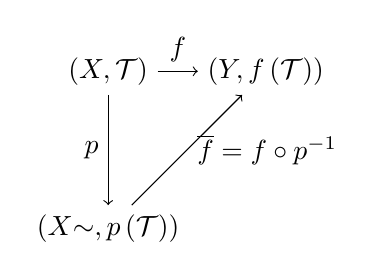
\begin{tikzpicture}[node distance=2cm, auto]
        \node(X) {$\left( X, \mathcal{T} \right)$};
        \node(Y) [right of=X] {$\left( Y, f\left( \mathcal{T} \right) \right)$};
        \node(Z) [below of=X] {$\left( \faktor{X}{\sim}, p\left( \mathcal{T} \right) \right)$};
        \draw[->](X) to node {$f$}(Y);
        \draw[->](X) to node [left] {$p$}(Z);
        \draw[->](Z) to node [right=0.2] {$\overline{f} = f \circ p^{-1}$}(Y);
        \end{tikzpicture}  
        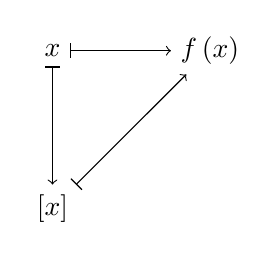
\begin{tikzpicture}[node distance=2cm, auto]
        \node(x) {$x$};
        \node(y) [right of=x] {$f\left( x \right)$};
        \node(z) [below of=x] {$\left[ x \right]$};
        \draw[|->](x) to (y);
        \draw[|->](x) to (z);
        \draw[|->](z) to (y);
        \end{tikzpicture}
        \caption{\textit{Representación de la composición del cociente}}
\end{figure}

\begin{obs}
La relación de equivalencia que vamos a usar es la que viene dada por la relación de \underline{inyectividad} respecto de $f$. Por esta razón, $\overline{f}$ será una biyección.
\end{obs}
\begin{demo}
Sea $z \in Y$ como $f$ es suprayectiva $\exists x \in X: f\left( x \right) = z$. A su vez, $y \in \left[ x \right] \Leftrightarrow f\left( x \right) = f\left( y \right) \Rightarrow \overline{f}\left( \left[ x \right] \right) = z$. Con esto, $\overline{f}$ es sobreyectiva y bien definida.

Sean ahora $\left[ x \right], \left[ y \right] \in \faktor{X}{\sim}$ tal que $\overline{f}\left[ x \right] = \overline{f}\left[ y \right] \Rightarrow f\left( x \right) = f\left( y \right) \Rightarrow \left[ x \right] = \left[ y \right]$. Por tanto, también es inyectiva.
\end{demo}

%TODO: No estoy seguro de como es esta proposición
\begin{prop}
\begin{enumerate}
    \item $\exists \overline{f} \Leftrightarrow x \sim y \Rightarrow f\left( x \right) \sim f\left( y \right)$
    \item $\exists \overline{f} : \overline{f}$ continua $\Leftrightarrow f$ continua.
    \item $\exists \overline{f}: \overline{f} \begin{cases}
        \text{sobre. }\\ 
        \text{iny. 1-1}\\ 
    \end{cases} \Leftrightarrow f \begin{cases}
        \text{sobre.}\\ 
        x \sim y \Leftarrow f \left( x \right) \sim f \left( y \right)
    \end{cases}$

    \item $\overline{f}$ homeomorfa $\Leftrightarrow f$ identificación.
    %TODO: Fix 
    \begin{figure}[H]
        \centering
        \begin{tikzpicture}[node distance=2cm, auto]
        \node(X) {$\left( X, \mathcal{T} \right)$};
        \node(Y) [right=2cm of X] {$\left( Y, \mathcal{T}' \right)$};
        \node(Z) [below=1.5cm of X] {$\left( \faktor{X}{\sim}, \overline{\mathcal{T}} \right)$};
        \draw[->](X) to node {$f$} node [below] {ident.}(Y);
        \draw[->](X) to node [left] {$p$} (Z);
        \draw[->](Z) to node [left=0.2] {$\overline{f}$} node [below=0.3] {homeo.} (Y);
        \end{tikzpicture}  
        \caption{\textit{Relación entre el cociente y una identificación.}}
        \label{fig:relacion_cociente_identificacion}
    \end{figure}
\end{enumerate} 
\end{prop}
\begin{demo}
\begin{enumerate}
    \item Por la definición de $\sim$ y de $\overline{f}$.
    %TODO: Corregir. Creo que se puede usar la propiedad universal
    \item Sea $\overline{f}$ continua. Tomemos $U \in \mathcal{T}' \Rightarrow \overline{f}^{-1}U \in \overline{\mathcal{T}}$. Como $p$ es continua por definición de $\overline{\mathcal{T}}$, $f^{-1} U = p^{-1} \overline{f}^{-1} U \in \mathcal{T}$. Por lo que $f$ es continua.

    Sea ahora $f$ continua. Tomemos $U \in \mathcal{T}' \Rightarrow W = f^{-1}U \in \mathcal{T}$. Al ser $p$ sobreyectiva $W = p^{-1}pW$, es decir, que $pW \in \overline{\mathcal{T}}$ (ya que $p^{-1}\left( p W \right) \in \mathcal{T}$ y la definición de $\overline{\mathcal{T}}$).

    \item (Anterior observación) Si $\overline{f}$ es inyectiva 1-1 $\Rightarrow \underbrace{\overline{f}\left[ x \right] = \overline{f}\left[ y \right]}_{\Leftrightarrow f\left( x \right) \sim f\left( y \right)} \Rightarrow \underbrace{\left[ x \right] = \left[ y \right]}_{\Leftrightarrow x \sim y}$
\end{enumerate}
\end{demo}

\begin{pg}
    Los cocientes son cómodos para definir espacios, las identificaciones son mejores para estudiar las propiedades que tenemos. Conviene pues tener triángulos como el anterior (\ref{fig:relacion_cociente_identificacion}). 

    Se puede contemplar $Y$ como un modelo del cociente. Es decir, utilizamos el cociente como ``modelo teórico'' y la identificación como ``modelo geométrico''. Esto no siempre será posible ya que dependerá de ciertas propiedades geométricas que veremos.
\end{pg}

\begin{ej}[Anteriores]
\begin{itemize}
    \item Circunferencia y el cilindro como cocientes:
    \begin{figure}[H]
        \centering
        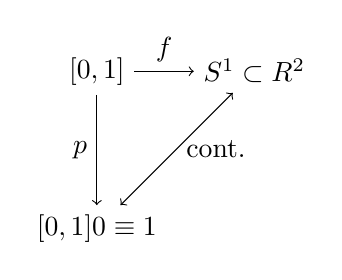
\begin{tikzpicture}[node distance=2cm, auto]
            \node(X) {$\left[ 0, 1 \right]$};
            \node(Y) [right of=X] {$\mathbb{S}^1 \subset \mathbb{R}^2$};
            \node(Z) [below of=X] {$\faktor{\left[ 0, 1 \right]}{0 \equiv 1}$};
            \draw[->](X) to node {$f$} (Y);
            \draw[->](X) to node [left] {$p$} (Z);
            \draw[<->](Z) to node [right] {cont.}(Y);
        \end{tikzpicture}
        %TODO: arreglar distancia X a Y
        \begin{tikzpicture}[node distance=2cm, auto]
            \node(X) {$\left[ 0, 1 \right] \times \left[ 0, 1 \right]$};
            \node(Y) [right=1.5cm of X] {$C \subset \mathbb{R}^3$};
            \node(Z) [below of=X] {$\faktor{\left[ 0, 1 \right] \times \left[ 0, 1 \right]}{\left( 0, t \right) \equiv \left( 1, t \right)}$};
            \draw[->](X) to (Y);
            \draw[->](X) to (Z);
            \draw[<->](Z) to (Y);
        \end{tikzpicture}
        \caption{\textit{En el primero tomamos un segmento de longitud $1$ y ``pegamos'' los extremos, lo que nos da una figura equivalente a un circunferencia. En el segundo, tomamos un rectángulo de área $1$ y ``pegamos'' el lado izquierdo con el derecho directamente.}}
    \end{figure}

    Para la circunferencia tenemos:
    \[
        \faktor{X}{\sim} = \left\{ \left\{ t \right\} : 0 < t < 1, \left\{ 0, 1 \right\} \right\}
    \]
    %TODO: Posiblemente mal
    la biyección entre el cociente y la esfera se da por el punto (3) de la anterior proposición y la continuidad por (2). Por último, la identificación se da por el anterior ejemplo.

    \item Para representar cocientes se utilizan dibujos que indican las identificaciones en los espacios de partida:
    \begin{figure}[H]
        \centering
        \hspace{2cm}
        \begin{tikzpicture}
            \node at (1,2.3) {Cilindro};
            \filldraw[color=cyan, fill=cyan!5, very thick,
                decoration={markings, mark=at position 0.18 with \arrow{>};,
                                      mark=at position 0.59 with \arrow{<};,
                           },
                postaction={decorate}
                ] (0,0) rectangle (2,2);
            \node[cyan] at (0,1.35) {\textbullet};
            \node[cyan] at (2,1.35) {\textbullet};
            \node[gray] at (2.1,1) [right] {$\left( 0, t \right) \equiv \left( 1, t \right)$};
        \end{tikzpicture}
        \begin{tikzpicture}
            \node at (1,2.3) {Banda de Möbius};
            \filldraw[color=cyan, fill=cyan!5, very thick,
                decoration={markings, mark=at position 0.18 with \arrow{>};,
                                      mark=at position 0.67 with \arrow{>};,
                           },
                postaction={decorate}
                ] (0,0) rectangle (2,2);
            \node[cyan](izq) at (0,1.35) {\textbullet};
            \node[cyan](der) at (2,0.67) {\textbullet};
            \node[cyan](O) at (1,1) {\textbullet};
            \draw[-, cyan, dashed] (izq) -- (der);
            \node[gray] at (2.1,1) [right] {$\left( 0, t \right) \equiv \left( 0, 1-t \right)$};
        \end{tikzpicture}
    \end{figure}
\end{itemize}
\end{ej}


\section{Productos (finitos)}%
\label{sec:productos_finitos_}
Supongamos que tenemos $p_i: X_1 \times \ldots X_r = \left( X_i, \mathcal{T}_i \right), 1 \le i \le r$ y buscamos hacerlas continuas. Trivialmente, podemos hacer que la topología en $X_i$ sea la discreta, sin embargo, esto carece de interés. Por esta razón, buscamos las topologías \underline{menos finas} que hagan $p_i$ continuas. 

Que $p_i$ sea continua quiere decir que $\forall U_i \in \mathcal{T}_i : U_i = X_1 \times \ldots U_i \times \ldots \times X_r$ debe ser abierto, es decir, que todos lo sean. Por tanto, $\bigcap_{i=1}^{r} p_i^{-1}U_i = U_1 \times \ldots \times U_r$ que son abiertos, pero no topología. Por tanto, definimos:
\begin{defi}
Llamamos \textbf{topología producto}, $\prod_{i=1}^{r} \mathcal{T}_i$, a aquella que viene determinada por la siguiente base:
\[
\mathcal{B} = \left\{ U_1 \times \ldots \times U_r: U_i \in \mathcal{T}_i \right\}
\]
\end{defi}

\begin{ej}
La $\mathcal{T}_u$ en $\mathbb{R}^n$ ese el producto de la usual en cada factor $\mathbb{R}$ de $\mathbb{R}^n$. La base de la definición de topología producto está formada por las ``bolas cuadradas''.
\end{ej}

\begin{theo}[Propiedad universal de la topología producto]
Sea $g: \left( Z, \mathcal{T}'' \right) \rightarrow \left( Y, \mathcal{T}' \right)$ y $p_i: \left( Y, \mathcal{T}' \right) \rightarrow \left( X_i, \mathcal{T}_i \right)$. Entonces:
    \[
    \mathcal{T}' = \prod_{i} \mathcal{T} \Leftrightarrow  
    \]
    \begin{equation}\label{eq:prop_universal_prod}
        \forall g \left[ g \text{ cont.} \Leftrightarrow \forall g_i \text{ cont.} \right]
    \end{equation}

    \begin{figure}[H]
        \centering    
            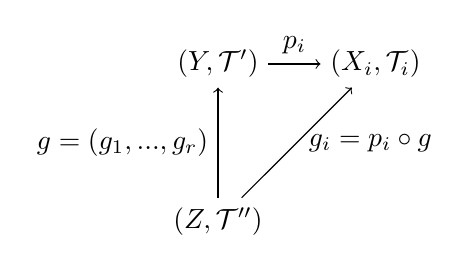
\begin{tikzpicture}[node distance=2cm, auto]
            \node(Y) {$\left( Y, \mathcal{T}' \right)$};
            \node(X) [right of=Y] {$\left( X_i, \mathcal{T}_i \right)$};
            \node(Z) [below of=Y] {$\left( Z, \mathcal{T}'' \right)$};
            \draw[->](Y) to node {$p_i$}(X);
            \draw[->](Z) to node [left] {$g = \left( g_1, ..., g_r \right)$}(Y);
            \draw[->](Z) to node [right=0.2ex] {$g_i = p_i \circ g$}(X);
            \end{tikzpicture}
        \caption{\textit{Ilustración de la composición propuesta}}
        \label{prop_universal_prod_finitos}
    \end{figure}
\end{theo}
\begin{demo}
\begin{enumerate}
    \item $\mathcal{T}' = \prod_{i} \mathcal{T}: $ 
    \begin{itemize}
        \item $g$ cont. $\Rightarrow g_i$ cont. (Composición de continuas)
        \item $g_i$ cont. $\Rightarrow g^{-1}\left( U_1 \times \ldots \times U_r \right) = \underbrace{g_1^{-1}\left( U_1 \right)}_{\mathcal{T}''} \cap \ldots \cap \underbrace{g_r^{-1}\left( U_i \right)}_{\mathcal{T}''} \in \mathcal{T}''$ (intersección finita de abiertos) 
    \end{itemize}

    \item Por otro lado,

    \begin{figure}[H]
        \centering    
            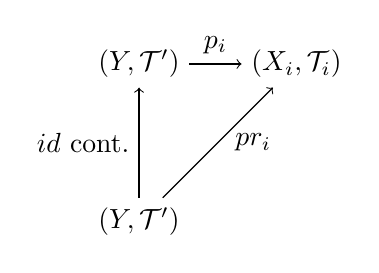
\begin{tikzpicture}[node distance=2cm, auto]
            \node(Y) {$\left( Y, \mathcal{T}' \right)$};
            \node(X) [right of=Y] {$\left( X_i, \mathcal{T}_i \right)$};
            \node(Z) [below of=Y] {$\left( Y, \mathcal{T}' \right)$};
            \draw[->](Y) to node {$p_i$}(X);
            \draw[->](Z) to node [right=0.1cm] {$pr_i$}(X);
            \draw[->](Z) to node [left] {$id$ cont.}(Y);
            \end{tikzpicture}
    \end{figure}
    Como $id$ será continua, aplicamos \ref{eq:prop_universal_prod} y tenemos que $g \circ p_i = pr_i$ es continua. Al ser $\prod_{i} \mathcal{T}_i $ la menos fina $\Rightarrow \mathcal{T}' \supset \prod_{i} \mathcal{T}_i$.

    \begin{figure}[H]
        \centering    
            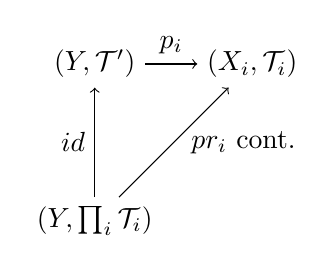
\begin{tikzpicture}[node distance=2cm, auto]
            \node(Y) {$\left( Y, \mathcal{T}' \right)$};
            \node(X) [right of=Y] {$\left( X_i, \mathcal{T}_i \right)$};
            \node(Z) [below of=Y] {$\left( Y, \prod_{i} \mathcal{T}_i \right)$};
            \draw[->](Y) to node {$p_i$}(X);
            \draw[->](Z) to node [right=0.1cm] {$pr_i$ cont.}(X);
            \draw[->](Z) to node [left] {$id$}(Y);
            \end{tikzpicture}
    \end{figure}
    Como $pr_i$ es continua por definición de $\prod_{i} \mathcal{T}_i$, aplicamos \ref{eq:prop_universal_prod} y tenemos que esta $id$ es continua. Por esta razón, $\prod_{i=1} \mathcal{T}_i \supset \mathcal{T}'$.
\end{enumerate}
\end{demo}

\begin{enun}
Demostrar (ii) sin usar que $\prod_{i} \mathcal{T}_i$ es la menos fina (usar que cumple la caracterización)
\end{enun}

\begin{prop}
\begin{enumerate}
    \item $p_i: Y \rightarrow X_i$ es abierta. 
    \item $X_j \xrightarrow{\alpha_j} Y: x_j \mapsto \left( a_1, \ldots, x_j, \ldots, a_r \right)$ es inmersión ($a_i \in X_i$ fijados).
\end{enumerate}
\end{prop}
\begin{demo}
\begin{enumerate}
    \item $p_i\left( U_1 \times \ldots \times U_r \right) = U_i$ 
    \item
    \[
    \begin{cases}
        \alpha_j\left( X_j \right) = \{a_1\} \times \ldots \times X_j \times \ldots \times \{a_r\} \\
        \alpha_j\left( U_j \right) = \{a_1\} \times \ldots \times U_j \times \ldots \times \{a_r\} = \alpha\left( X_j \right) \cap \left( X_1 \times \ldots \times U_j \times \ldots \times X_r \right) 
    \end{cases}
    \]
\end{enumerate}
\end{demo}

\begin{pg}
En una topología producto ``todo se genera en productos''.
\begin{ej}
\begin{itemize}
    \item Bases de entornos: $\mathcal{V}^a = \mathcal{V}^{a_1} \times \ldots \times \mathcal{V}^{a_r} \stackrel{mut??}{=} \{V_1 \times \ldots \times V_r: V_i \in \mathcal{V}^{a_i}\} \left( a \in Y \right)$.
    \item Base de abiertos: $\mathcal{B} = \mathcal{B}_1 \times \ldots \times \mathcal{B}_r = \{B_1 \times \ldots \times B_r: B_i \in \mathcal{B}_i\}$ (esto repite la construcción de $\prod_{i} \mathcal{T}_i$)
\end{itemize}
\end{ej}
\end{pg}


\section{Sumas (finitas)}%
\label{sec:sumas_finitas}
Supongamos que tenemos $e_i: \left( X_i, \mathcal{T}_i \right) \rightarrow X_1 + \ldots + X_r = \left( X_1 \times \left\{ 1 \right\} \right) \cup \ldots \cup \left( X_r \times \left\{ r \right\} \right), 1 \le i \le r: x_i \mapsto \left( x_i, i \right)$ y buscamos hacerlas continuas. Trivialmente, podemos hacer que la topología en $Y$ sea la trivial, sin embargo, esto carece de interés. Por esta razón, buscamos la topología \underline{más fina} que haga $f$ continua.

Debido a que, $\forall U_i \in \mathcal{T}_i,\ e_i^{-1}\left( U_i \times \left\{ i \right\} \right)$, podemos definir lo siguiente:
\begin{defi}
Llamamos \textbf{topología suma}, $\sum_{i=1}^{k} \mathcal{T}_i$, a aquella que viene determinada por la siguiente base:
\[
\mathcal{B} = \left\{ U_1 \times \left\{ 1 \right\}, \ldots, U_r \times \left\{ r \right\}: U_i \in \mathcal{T}_i \right\}
\]
\end{defi}

\begin{prop}
Con la anterior definición sabemos que 
\[
e_i: \left( X_i, \mathcal{T}_i \right) \rightarrow \left( X_i\times \{i\}, \mathcal{T}|_{X_i \times \{i\}} \right),\ \forall i \in \left\{ 1, \ldots, r \right\}
\]
es inmersión abierta y cerrada.
\end{prop}
\begin{demo}
\begin{itemize}
    \item Inmersión abierta: $e_i\left( U_i \right) = U_i \times \{i\} \in \mathcal{T}$
    \item Cerrada: $Y\setminus e_i\left( X_i \right) = Y \setminus X_i \times \{i\} = \bigcup_{j \neq i} X_j \times \{j\} \in \mathcal{T}$
\end{itemize}
\end{demo}

%TODO: Fix teorema
\begin{theo}[Caracterización topología suma]
Sea $g: \left( Y, \mathcal{T}' \right) \rightarrow \left( Z, \mathcal{T}'' \right)$ y $e_i: \left( X_i, \mathcal{T}_i \right) \rightarrow \left( Y, \mathcal{T}' \right)$. Entonces:
    \[
    \mathcal{T}' = \mathcal{T}_1 + \ldots + \mathcal{T}_r \Leftrightarrow  
    \]
    \begin{equation}\label{eq:prop_universal_sum}
        \forall g \left[ g \text{ cont.} \Leftrightarrow \forall g_i \text{ cont.} \right]
    \end{equation}

    \begin{figure}[H]
        \centering    
            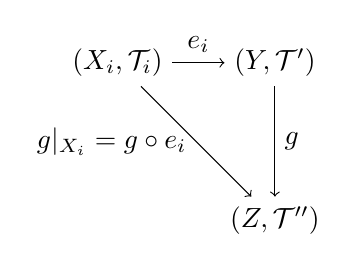
\begin{tikzpicture}[node distance=2cm, auto]
            \node(X) {$\left( X_i, \mathcal{T}_i \right)$};
            \node(Y) [right of=X] {$\left( Y, \mathcal{T}' \right)$};
            \node(Z) [below of=Y] {$\left( Z, \mathcal{T}'' \right)$};
            \draw[->](X) to node {$e_i$}(Y);
            \draw[->](X) to node [left] {$g|_{X_i} = g \circ e_i$}(Z);
            \draw[->](Y) to node {$g$}(Z);
            \end{tikzpicture}
        \caption{\textit{Ilustración de la composición propuesta}}
        \label{prop_universal_sum_finitas}
    \end{figure}
\end{theo}
%TODO: Tal vez hacerlo bien?
\begin{demo}
    Análoga a las anteriores construcciones.
\end{demo}

\begin{pg}
Localmente $Y = X_1 + \ldots + X_r$ es como sea cada $X_i$. Por ejemplo, las bases de entornos de $Y$ son las de los sumandos. Globalmente, se trata cada sumando separadamente. Por ejemplo, las bases de abiertos de los sumandos se unen para dar una base de abiertos de $Y$. Olvidando el tecnicismo $X_i \times \{i\} \equiv X_i$:
\begin{center}
   $Y$ es unión disjunta de los sumandos\\
   Los sumando son subespacios abiertos y cerrados de $Y$
\end{center}
Es un formalismo para hacer cómodamente otras construcciones. Por ejemplo, ``pegar dos discos por sus bordes'' sería:
\begin{gather*}
    \text{Disco } D \subset \mathbb{R}^2: x^2 + y^2 \le 1, \text{ borde } \partial D = \mathbb{S}^1: x^2 + y^2 = 1\\
    %TODO: Fix cociente
    \faktor{D_1 + D_2}{\sim} \quad \overbrace{\left( p, 1 \right)}^{\in \partial D} \sim \left( p, 2 \right) 
.\end{gather*}

\begin{figure}[H]
    \centering
    \incfig{dos-discos.}
    \caption{\textit{Dos discos}}
    \label{fig:dos-discos.}
\end{figure}
y más elaborado $h: \partial D \stackrel{\text{homeo.}}{\approx} \partial D$ con $\overbrace{p}^{\in \partial D} \sim h\left( p \right)$.

Finalmente, hay otros conceptos de ``suma'' más significativos que veremos en algún ejemplo.
\end{pg}


\section{Espacios proyectivos reales}%
\label{sec:espacios_proyectivos_reales}
\subsection{Geometría lineal}
\label{sub:geometría_lineal}
En primer lugar, veamos un repaso de lo visto en geometría lineal sobre espacios proyectivos.
\begin{defi}[Espacio proyectivo real]    
Usando $\sim$, proporcionalidad: 
\[
\mathbb{R}P^n = \mathbb{P}^{n} = \faktor{\mathbb{R}^{n+1}\setminus \{0\}}{\sim} \Rightarrow \mathbb{P}^{n} = \{\text{rectas vectoriales de } \mathbb{R}^{n+1}\}     
\]
Que en coordenadas es:
\begin{align*}
    \pi: \mathbb{R}^{n+1} \setminus \{0\} &\rightarrow \mathbb{P}^{n}\\
    \left( x_0, \ldots, x_n \right) &\mapsto \left( x_0 : \ldots : x_n \right) 
.\end{align*}
\end{defi}
\begin{obs}
Las ecuaciones serán de la forma: $h\in \mathbb{R}\left[ x_0, \ldots, x_n \right]$ homogénea $\Rightarrow \begin{cases}
    h\left( x \right) = 0\\
    h\left( x \right) \neq 0
\end{cases}$ está bien definido en $\mathbb{P}^{n}$.
Sabemos que el grado de la ecuación homogénea $h$ nos dará lugar a:
\begin{itemize}
    \item Grado \underline{1}: Variedades proyectivas lineales.
    \item Grado \underline{2}: Cuádricas proyectivas.
    \item Grado \underline{arbitrario}: Variedades proyectivas algebraicas.
\end{itemize}
\end{obs}

\begin{defi}[Cartas afines]
Sea $H \subset \mathbb{P}^n$ un hiperplano proyectivo. Entonces, tenemos un hiperplano lineal $\hat{H} \subset \mathbb{R}^{n+1}$, con una forma lineal asociada $h = 0$, de la siguiente forma:
\[
H = \faktor{\hat{H}\setminus \left\{ 0 \right\}}{\sim}
\]
Decimos que $H$ es \textbf{hiperplano del infinito} de la \textbf{carta afín} $U = \mathbb{P}^n \setminus H$.
\end{defi}
\begin{prop}
La aplicación 
\[
\pi|: \underbrace{\left\{ h = 1 \right\}\subset \mathbb{R}^{n+1} \setminus \left\{ 0 \right\}}_{\text{Hiperplano afín}} \rightarrow \underbrace{\mathbb{P}^{n} \setminus H}_{\left\{ h \neq 0 \right\}} = U
\]
es una biyección.
\end{prop}

\subsection{Topología de espacio proyectivos}
\label{sub:topología_de_espacio_proyectivos}
Para la topología en $U$ usaremos la imagen directa de la usual en $\left\{ h = 1 \right\} \subset \mathbb{R}^{n+1}$
\begin{prop}
Con la anterior suposición tenemos que la aplicación:
\[
\pi|: \{h = 1\} \rightarrow U
\]
es un \underline{homeomorfismo}.     
\end{prop}
\begin{demo}
Ya sabemos que es biyección por lo que queda ver que es continua y abierta/cerrada. Continua lo será por tener $U$ la topología imagen directa. Y abierta porque???%TODO
\end{demo}
%TODO: Creo que esta demostración no es de esto.
%\begin{demo}
%Veamos lo que tenemos:
%\begin{figure}[H]
%    \centering
%        \begin{tikzpicture}[node distance=2cm, auto]
%        \node(X) {$\mathbb{R}^{n+1} \setminus \left\{ 0 \right\}$ usual};
%        \node(Z) [below of=X] {$U \subset \mathbb{P}^n$ cociente};
%        \node(Y) [left=1.2cm of Z] {$\mathbb{R}^{n+1} \supset \left\{ h = 1 \right\}$};
%        \draw[->](X) to node [left] {$\pi$}(Z);
%        \draw[->](Y) to node [below] {homeo.}(Z);
%        \end{tikzpicture}
%    \captionsetup{font={color=gray}}
%    \caption[gray]{\textit{Composición propuesta}}
%    \label{}
%\end{figure}
%Tomemos $W \subset U \begin{cases}
%    \text{cociente: } \pi^{-1} \left( W \right) \stackrel{\text{ab.}}{\subset} \mathbb{R}^{n+1} \setminus \left\{ 0 \right\}\\
%    \text{homeo: } \pi^{-1}\left( W \right) \cap \left\{ h = 1 \right\} \stackrel{\text{ab.}}{\subset} \left\{ h=1 \right\}
%\end{cases}$.    
%Cociente $\Rightarrow$ homeomorfismo es trivial y significa que $\pi|_{\left\{ h=1 \right\}}$ es continua. Homeomorfismo $\Rightarrow$ cociente porque:
%\[
%\pi^{-1}\left( W \right) = \text{cono de } \underbrace{\pi^{-1}\left( W \right) \cap \left\{ h = 1 \right\}}_{A}
%\]
%Como $\left\{ h=1 \right\} \supset A$ abierto $\Leftrightarrow \text{cono}\left( A \right) \stackrel{\text{ab.}}{\subset} \mathbb{R}^{n+1} \setminus \left\{ 0 \right\}$ donde cono$\left( A \right) = \left\{ \lambda a: a \in A, \lambda \in \mathbb{R} \setminus \left\{ 0 \right\} \right\}$
%\end{demo}

\begin{prop}
La siguiente definición es topología en $\mathbb{P}^n$:
\[
W \text{ abierto si } W \cap U \text{ es abierto } \forall U \text{ carta afín.}
\]
\end{prop}
\begin{demo}
%TODO
Ni idea
\end{demo}

%TODO: Fix topologia
\begin{prop}[Topología en Pn]    
\begin{itemize}
    \item \underline{Cociente} de la usual vía $\mathbb{R}^{n+1}\setminus \{0\} \xrightarrow{\pi} \mathbb{P}^{n}: \left( x_0, \ldots, x_n \right) \mapsto \left( x_0 : \ldots : x_n \right)$
    \item ``\underline{Suma}'' de las definidas en las cartas afines:
    \[
        W \text{ abierto si } W \cap U \text{ es abierto } \forall U \text{ carta afín.} 
    \]
\end{itemize}
Estas dos topologías coinciden.
\end{prop}
\begin{demo}
\begin{enumerate}
    \item $U$ es abierto en la topología cociente ya que $\pi^{-1} U = \{h \neq 0\}$ es abierto usual.
    \item La topología cociente en $U$ coincide con la topología de carta afín:
    %¡¡¡¡IMPORTANTE!!!!: TOCAR LO MINIMO POSIBLE
    \begin{figure}[H]
        \centering
        \begin{tikzpicture}
            \node(top) at (0,0) {$W \subset U : \pi^{-1}W = $ cono sobre $\underbrace{\left( \pi^{-1} W \right)\cap \left\{ h = 1 \right\}}_{= \left( \pi|_{\left\{ h=1 \right\}} \right)^{-1}W}$}; 
            %Izquierda
            \draw[->] (-2.4,0) -- (-2,0.1);
            \node at (-2,0) [below, text width=2cm] {para la top. cociente};
            %Derecha
            \draw[->] (4.4,-0.3) -- (3.5,-0.3);
            \node at (5.5,0.2) [below, text width=2cm] {para la top. de carta afín};

            \draw[-{implies},double] (0,0) -- (0,-2);

            \node(bottom) at (0.7,-2.2) {$\pi^{-1}W \stackrel{\text{ab.}}{\subset} \mathbb{R}^{n+1} \Leftrightarrow \left( \pi|_{\left\{ h=1 \right\}}^{-1} \right)W \stackrel{\text{ab.}}{\subset}\left\{ h=1 \right\}$};

            %Izquieda
            \draw[implies-implies,double] (-1.35,-2.4) -- (-1.35,-3);
            \node at (-1.35,-3) [below, text width=2cm] {$W$ abierto top. cociente};
            %Derecha
            \draw[implies-implies,double] (2.55,-2.4) -- (2.55,-3);
            \node at (2.55,-3) [below, text width=2cm] {$W$ abierto top. carta afín};
        \end{tikzpicture}
        \captionsetup{font={color=gray}}
        \caption[gray]{\textit{Equivalencia entre las topologías cociente y suma.}}
        \label{fig:cociente_suma_equivalentes}
    \end{figure}
    \item[1. + 2.] $\Rightarrow $ La top. cociente está generada por las topologías de las cartas afines, que forman un recubrimiento abierto de $\mathbb{P}^{n}$.
\end{enumerate}
\end{demo}

%TODO: Fix orden
\begin{prop}
    En este caso, la $\mathcal{T}_{\text{cociente}}$ tendrá como base: $\left\{ \pi\left( B \right) \subset U : B \stackrel{\text{ab.}}{\subset} \left\{ h = 1 \right\},\ h \in \mathbb{P}\left[ x_0, \ldots, x_n \right] \right\}$ homogéneo de grado $1: G = \bigcup_{U} G \cap U$ abierto en $\mathbb{P}^n$ y abierto en $U$.
\end{prop}

\begin{obs}
    En $U_1 \cap U_2$ la topología definida por $\pi_1 = $ definida por $\pi_2$.
\end{obs}

\begin{obs}
De lo anterior deducimos:
\begin{enumerate}
    \item $U_1, U_2$ dos cartas afines $\Rightarrow U_1 \cap U_2$ abiertos.
    \begin{demo}
    \[
        \text{Cartas afines: } U_i = \{h_1 \neq 0\} \begin{cases}
                \pi|: \{h_1 = 1\} \rightarrow U_1 \text{homeo.}\\
                \left( \pi_1 \right)^{-1}\left( U_1 \cap U_2 \right) = \{h_1 = 1, h_2 \neq 0\} \stackrel{\text{ab.}}{\subset} \{h_1 = 1\}  
        \end{cases}  
    \]
    \end{demo}
    \item Las topologías de $U_1$ y $U_2$ coinciden en $U_1 \cap U_2$.
    \begin{demo}
        De nuevo conviene entenderlo con cartas:
        %TODO: Fix
        \begin{center}
            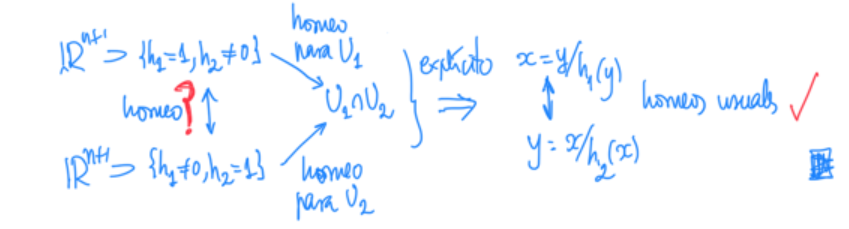
\includegraphics[scale=0.3]{images/obs_cartas_afines} 
        \end{center}
    \end{demo}
\end{enumerate}
\end{obs}

%TODO: Esto es posible que se pueda agrupar mejor (hasta Möbius)
\begin{defi}[Atlas afín canónico]
No se suelen utilizar todas las cartas afines: $n + 1$ distintas ya cubren $\mathbb{P}^{n}$. Típicamente $\mathbb{P}^{n} = U_0 \cup \ldots \cup U_n$ con:
\[
    U_i = \{x_i \neq 0\} \leftrightarrow \{\underbrace{x_i = 1}_{\equiv \mathbb{R}^n}\}: \left( x_0 : \ldots : x_i : \ldots : x_n \right) \mapsto \left( \frac{x_0}{x_i}, \ldots, \underbrace{\not1}_{\mathbb{R}^n \rightarrow}, \ldots, \frac{x_n}{x_i} \right), 0 \le i \le n
\]
\end{defi}

\begin{prop}[Cociente antipodal]
    Toda recta de $\mathbb{R}^{n + 1}$ corta a $\mathbb{S}^{n}: x_0^2 + \ldots + x_n^2 = 1$ en dos puntos \underline{antipodales}, así que denotamos un ``sub'' cociente, que es también identificación.
    \begin{figure}[H]
        \tikzset{
            draw=none,
            subset/.style={
                edge node={node [sloped, allow upside down, auto=false]{$\subseteq$}}
            }
        }
        \centering
            \begin{tikzpicture}[node distance=2cm, auto]
            \node(X) {$\mathbb{R}^{n+1}\setminus \left\{ 0 \right\}$};
            \node(Y) [right=0.2cm of X] {$\mathbb{S}^n$};
            \node(Z) [below of=X] {$\mathbb{R}^n$};
            \node at (1.03,-0.01) {$\supset$};
            \draw[->](X) to (Z);
            \draw[->](Y) to node [right] {$\pi|$} (Z);
            \end{tikzpicture}
        \caption{\textit{Cociente antipodal de $\mathbb{S}^n$}}
        \label{fig:cociente_antipodal_Sn}
    \end{figure}
\end{prop}
\begin{demo} 
    Como antes tenemos conos: $\pi^{-1}W = $ cono sobre $\underbrace{\mathbb{S}^n \cap \pi^{-1}W}_{= \left( \pi / \mathbb{S}^n \right)^{-1} W}$.
\end{demo}
\begin{obs}
    Las cartas afines tienen una representación muy conveniente:
    %TODO: Fix imagen
    \begin{center}
        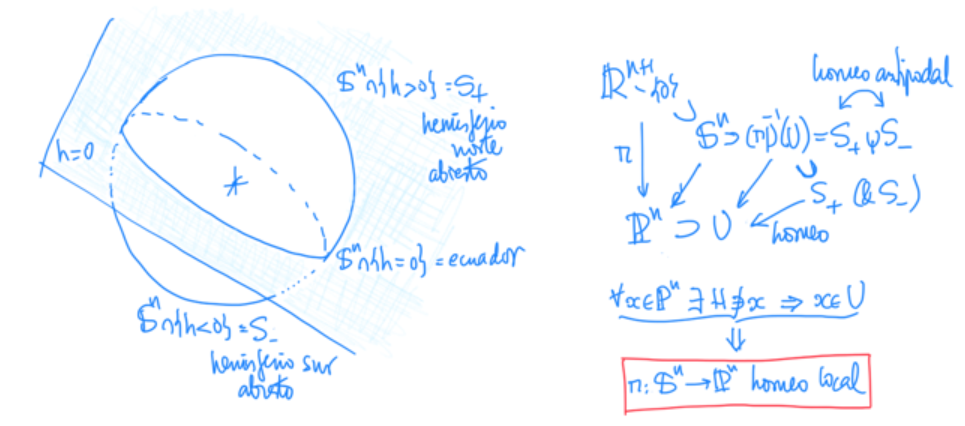
\includegraphics[scale=0.3]{images/repr_carta_afin} 
    \end{center}
\end{obs}

%TODO: Demostrar que un hemisferio tiene una identificación al proyectivo. 
\begin{prop}[Cociente de un disco]
Consideremos un disco:
\[
    E = \{h = 0, x_0^2 + \cdots + x_n^2 = 1\} = \partial \begin{cases}
        \overline{S}_+ = \mathbb{S}^n \cap \{h \ge 0\} \text{ hemisferio cerrado.} \\
        D^n = \{h = 0, x_0^2 + \cdots + x_n^2 \le 1\} \text{ disco.} 
    \end{cases} 
\]
%TODO: Fix imagen
\begin{center}
    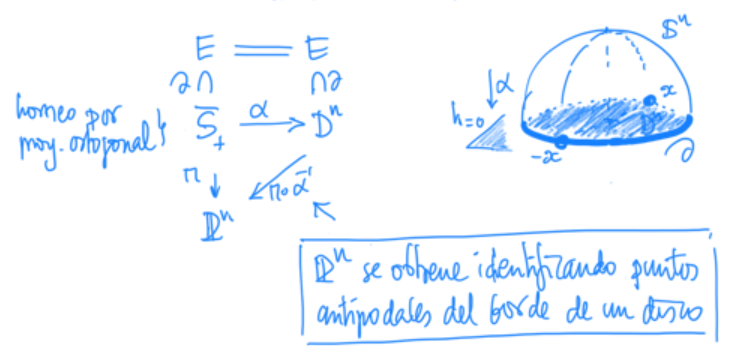
\includegraphics[scale=0.3]{images/cociente_disco} 
\end{center}
\end{prop}

\begin{ej}
$\mathbb{P}^{2} \setminus D^2 = $ banda de Möbius.
%TODO: Fix imagen
\begin{center}
    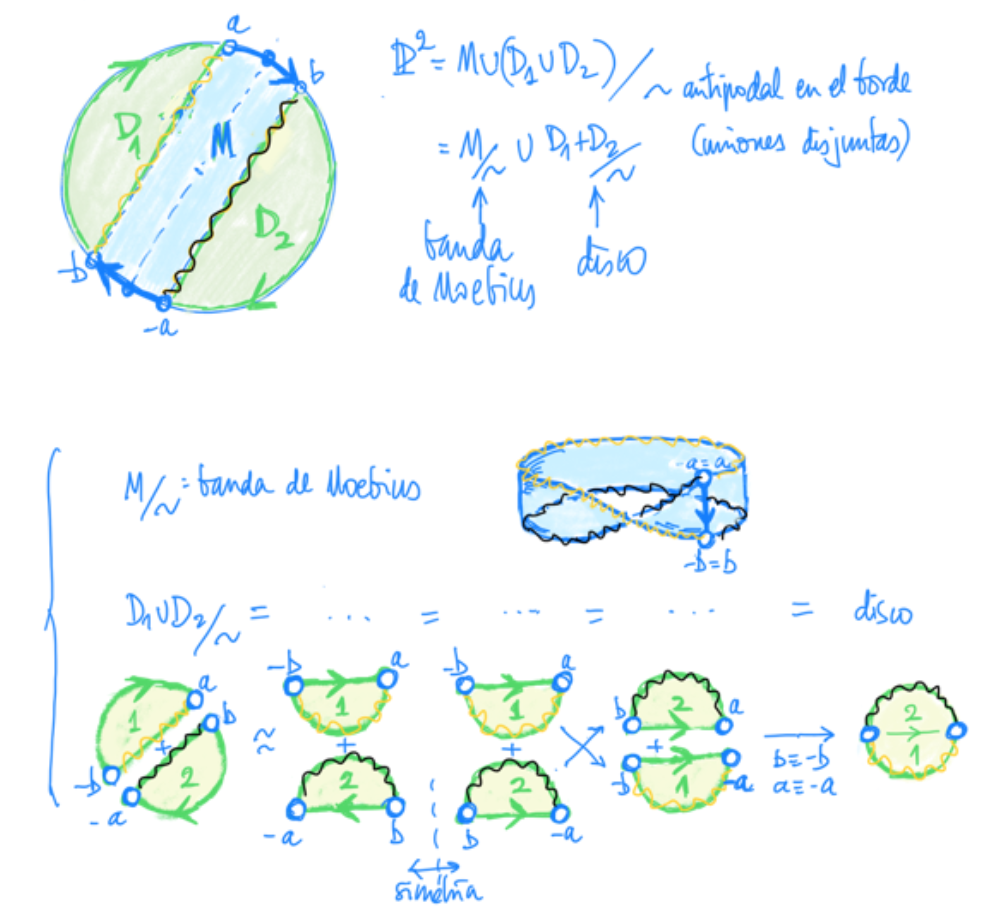
\includegraphics[scale=0.3]{images/banda_moebius} 
\end{center}
\end{ej}

